\documentclass[review]{elsarticle}
\usepackage[utf8]{vietnam}
\setlength{\parskip}{10pt}
%\usepackage[pdftex]{graphicx}
%\usepackage[font=footnotesize]{caption}

\usepackage{mwe}    % loads »blindtext« and »graphicx«
\usepackage{subfig}
\usepackage{array}
\usepackage{float}
\usepackage{subfloat}
\usepackage{sidecap}

\usepackage{epstopdf}

\usepackage{mathtools}

\usepackage{lineno,hyperref}
\modulolinenumbers[5]

\journal{Journal of \LaTeX\ Templates}

%%%%%%%%%%%%%%%%%%%%%%%
%% Elsevier bibliography styles
%%%%%%%%%%%%%%%%%%%%%%%
%% To change the style, put a % in front of the second line of the current style and
%% remove the % from the second line of the style you would like to use.
%%%%%%%%%%%%%%%%%%%%%%%

%% Numbered
%\bibliographystyle{model1-num-names}

%% Numbered without titles
%\bibliographystyle{model1a-num-names}

%% Harvard
%\bibliographystyle{model2-names.bst}\biboptions{authoryear}

%% Vancouver numbered
%\usepackage{numcompress}\bibliographystyle{model3-num-names}

%% Vancouver name/year
%\usepackage{numcompress}\bibliographystyle{model4-names}\biboptions{authoryear}

%% APA style
%\bibliographystyle{model5-names}\biboptions{authoryear}

%% AMA style
%\usepackage{numcompress}\bibliographystyle{model6-num-names}

%% `Elsevier LaTeX' style
\bibliographystyle{elsarticle-num}
%%%%%%%%%%%%%%%%%%%%%%%

\begin{document}

\begin{frontmatter}

\title{Pseudo-3D Trajectories: An Effective Approach for Motion Representation in Depth Data}

%% Group authors per affiliation:
\author{Chien-Quang LE}
\address{The Graduate University for Advanced Studies}

%% or include affiliations in footnotes:
\author{Duy-Dinh LE}
\address{National Institute of Informatics}

\author{Shin'ichi Satoh}
\address{National Institute of Informatics}


\begin{abstract}
Leveraging the motion information of trajectories shows the effectiveness to the human action recognition in 2D video. However, the issue is that this approach direction is effective or not when represents motions in 3D video is not still answered. In this paper, we will deal with this issue by conducting experiments based on 2D trajectory features to present motion information from one 3D video representation. Beside, in order to ensure including depth information, we propose a method based on compensating motion information from other representations. Evaluated on the benchmark datasets, our method significantly outperforms the 3D SoA methods.
\end{abstract}

\begin{keyword}
\texttt{Trajectory}\sep action recognition\sep depth\sep feature representation
%\MSC[2010] 00-01\sep  99-00
\end{keyword}

\end{frontmatter}

\linenumbers

\section{Introduction}

\paragraph{Background and Challenges} Gần đây, với sự phát triển của RGB-D camera như Kinect, depth data đã mở ra nhiều hướng nghiên cứu tiềm năng cho bài toán Human Action Recognition. So sánh với intensity images thông thường, depth maps hỗ trợ nhiều advantages hơn. Ví dụ, depth maps cung cấp các thông tin về shape rõ ràng hơn so với intensity images. Hơn thế nữa, depth data ít bị ảnh hưởng bởi những thay đổi của ánh sáng. Tuy nhiên, các phương pháp dựa trên intensity liệu có hiệu quả trên depth data hay không vẫn chưa được quan tâm nhiều.

\paragraph{Existing approaches and drawbacks} Trong bài toán action recognition, để adapt các phương pháp dựa trên intensity cho depth data có 2 yếu tố chính. Thứ nhất, để capture motion information hiệu quả việc chọn lựa a robust feature representation là rất quan trọng. Thứ hai, để đảm bảo motion là đầy đủ thông tin trong depth video, việc bổ sung thông tin depth vào feature representation là yêu cầu không thể thiếu. Tuy nhiên, các phương pháp được đề xuất gần đây vẫn chưa hội tụ đủ 2 yếu tố này. Một số phương pháp như \cite{yang2012recognizing, xia2013spatio} xem xét depth value như là intensity value và adapt các intensity-based techniques. Mặc dù, chúng có thể đạt được những kết quả hợp lý, nhưng tất cả chúng đều phải đối mặt với nhiều hạn chế. [DMM-HOG] có thể tận dụng thông tin depth từ các phép chiếu của depth maps. Nhưng its feature representation dựa trên global motion như HOG sẽ dễ gây nhầm lẫn bởi những similar postures. \cite{xia2013spatio} có thể đảm bảo depth information trong việc tính toán features. Nhưng cách tiếp cận này không đảm bảo được sự tin cậy khi extract các local points, do bởi textureless data and depth noise. Ngoài hướng tiếp cận trên, các phương pháp như \cite{wang2012mining, oreifej2013hon4d} chỉ tập trung khai thác depth information nên không tận dụng được sức mạnh của các intensity-based features. Do đó, hướng nghiên cứu của chúng tôi là propose một phương pháp có thể đáp ứng đầy đủ cả 2 yếu tố nêu trên.

\paragraph{Proposal, Idea and Steps}Trong bài báo này, chúng tôi sử dụng một feature representation dựa trên dense trajectories của \cite{wang2011densetraj}, do bởi hiệu quả của cách tiếp cận này trong nhiều bài toán, including activity recognition and multimedia event detection. Các trajectories thu được bằng cách tracking các sampled points densely sử dụng optical flow fields. Sau khi extract trajectories, các trajectory-aligned descriptors sẽ được adopted. Sau đó, features tính toán được từ các descriptors này sẽ được sử dụng cho việc biểu diễn motion information trong video.

Tuy nhiên, việc thiếu sót depth information trong feature representation có thể gây ra các trường hợp bị confused, như được chỉ ra trong Figure \ref{subfig-1:FrontView}. Do đó, để đảm bảo việc không bỏ sót thông tin depth, ý tưởng cơ bản là combine thông tin chuyển động từ nhiều góc nhìn khác nhau. Các biểu diễn từ nhiều góc nhìn có thể đạt được bằng cách chiếu depth maps lên trên các mặt phẳng tương ứng. Việc chiếu này dễ dàng thực hiện được bởi những thuận lợi mà depth data mang lại.

\begin{figure}[H]
	\begin{center}
		\subfloat[From front view\label{subfig-1:FrontView}]{ %
			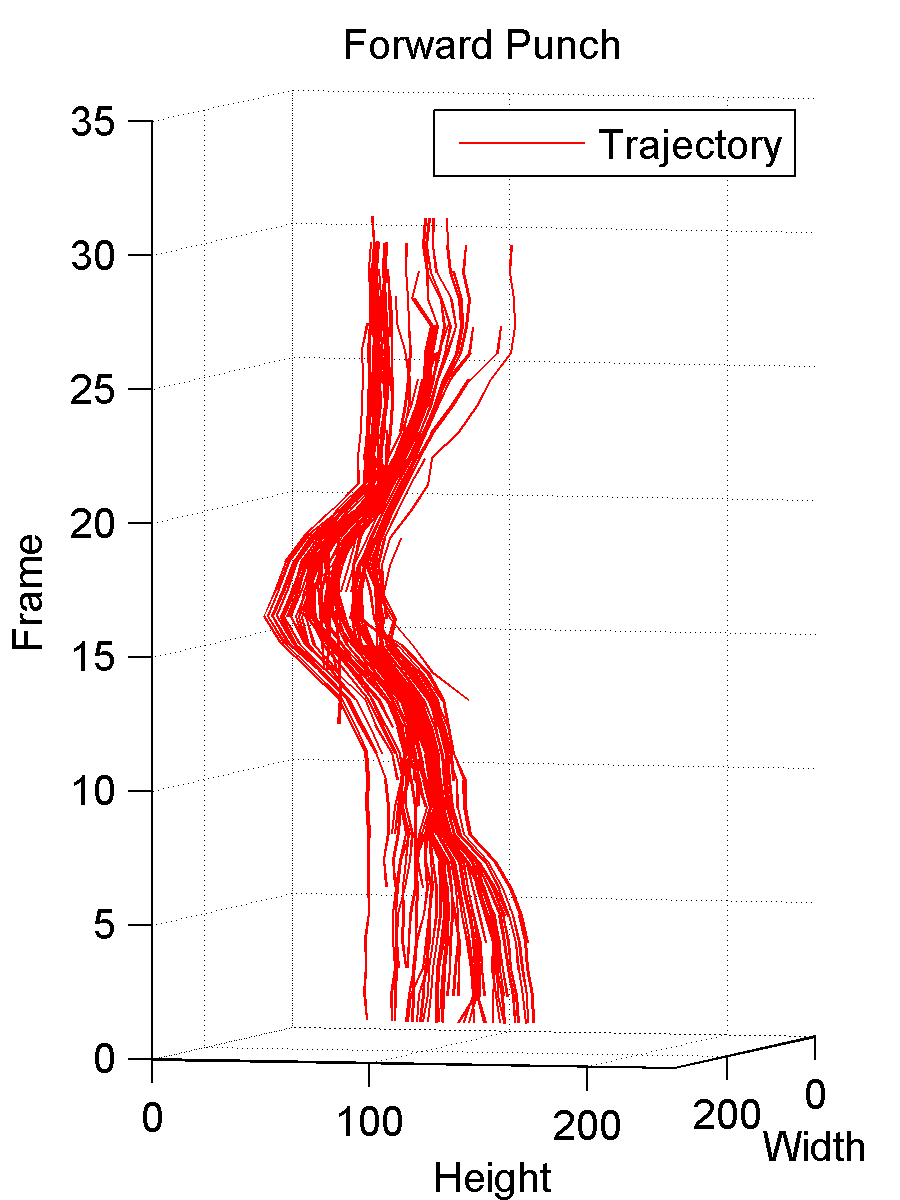
\includegraphics[scale=0.5]{ForwardPunch_FRONT.png}
			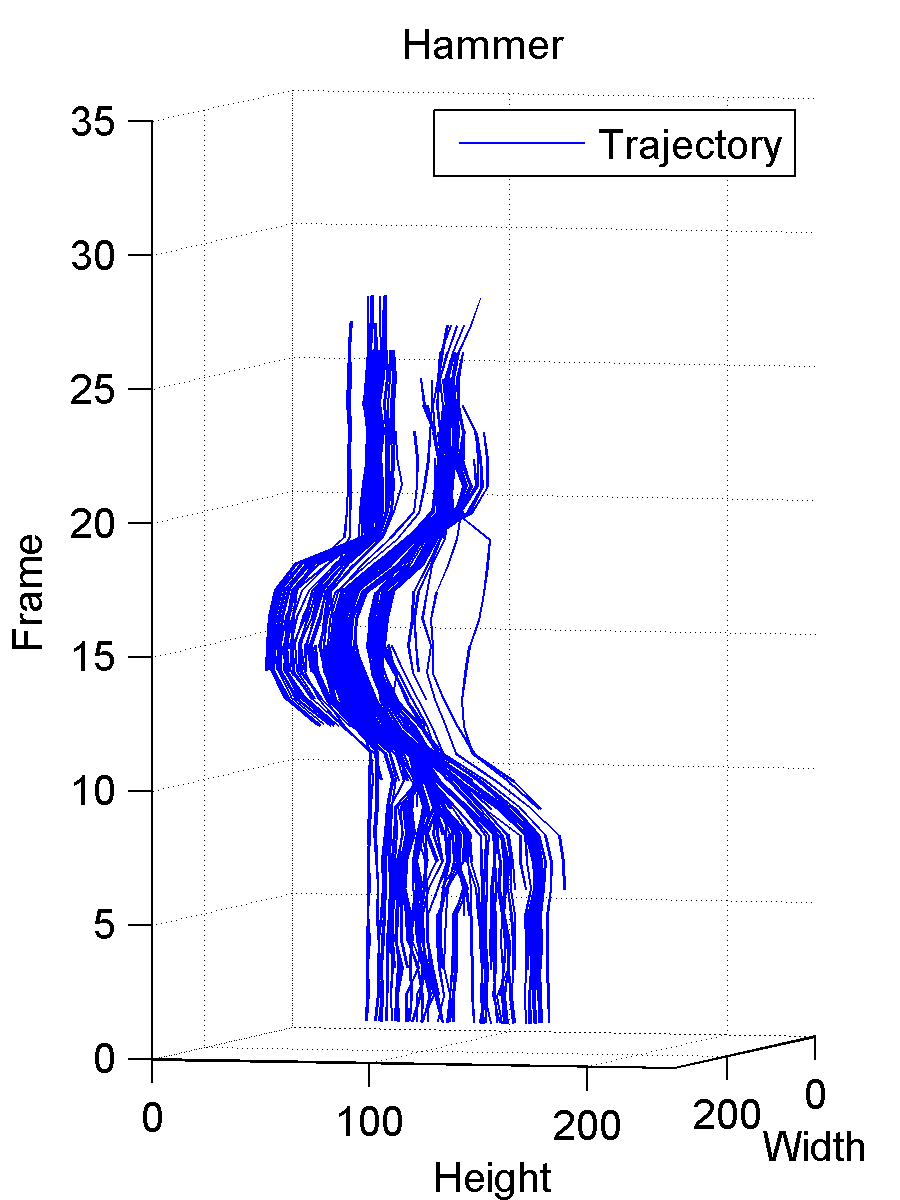
\includegraphics[scale=0.5]{Hammer_FRONT.png}
		}
	\end{center}
	\begin{center}
		\subfloat[From side view\label{subfig-2:SideView}]{ %
			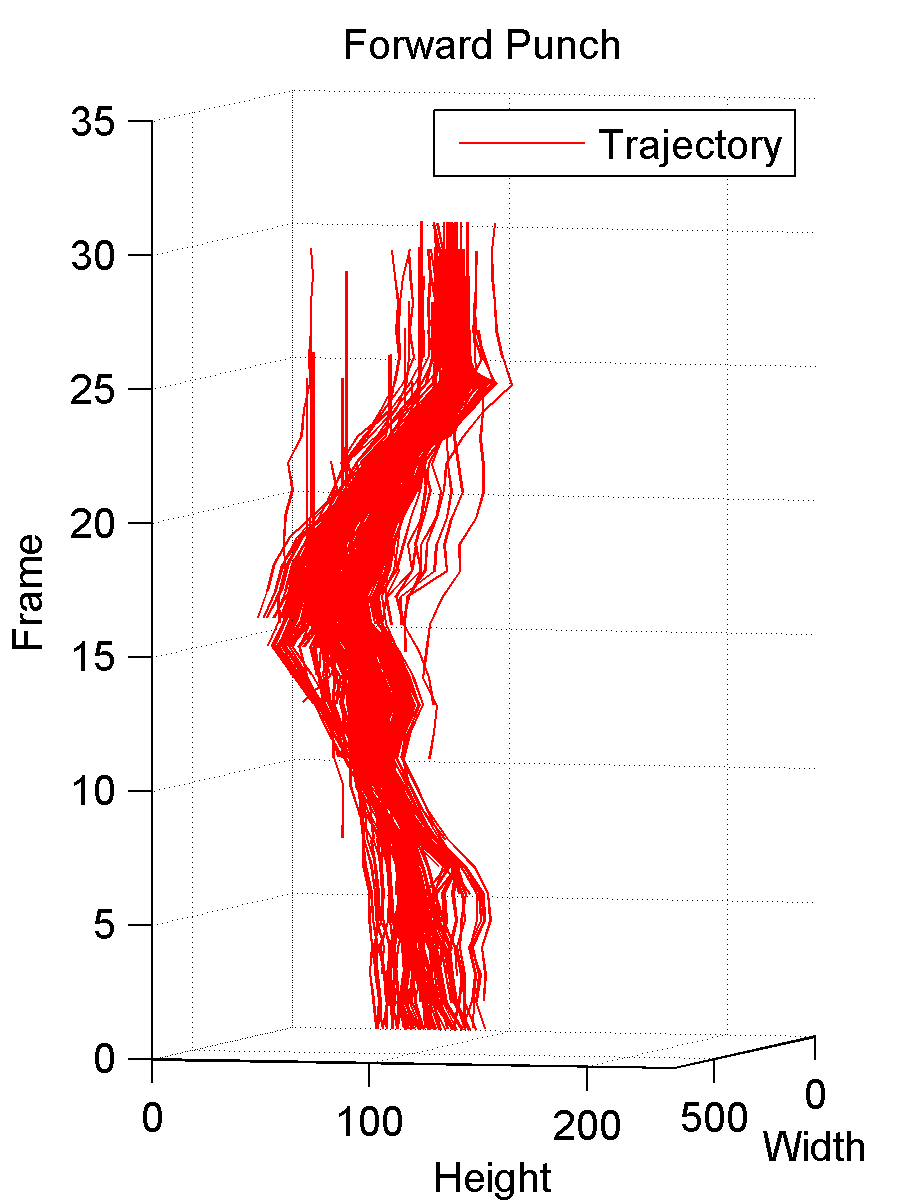
\includegraphics[scale=0.5]{ForwardPunch_SIDE.png}
			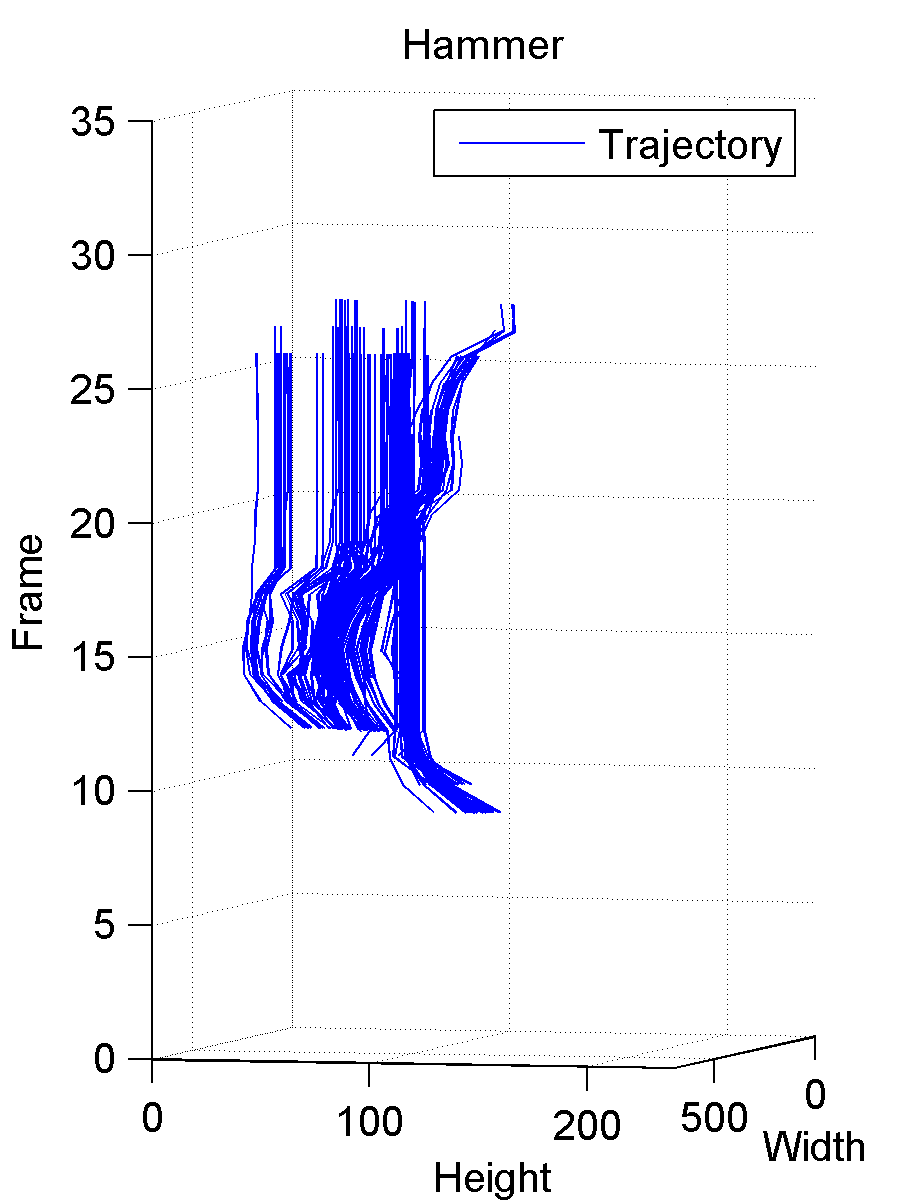
\includegraphics[scale=0.5]{Hammer_SIDE.png}
		}
	\end{center}
	\begin{center}
		\subfloat[From top view\label{subfig-3:TopView}]{ %
			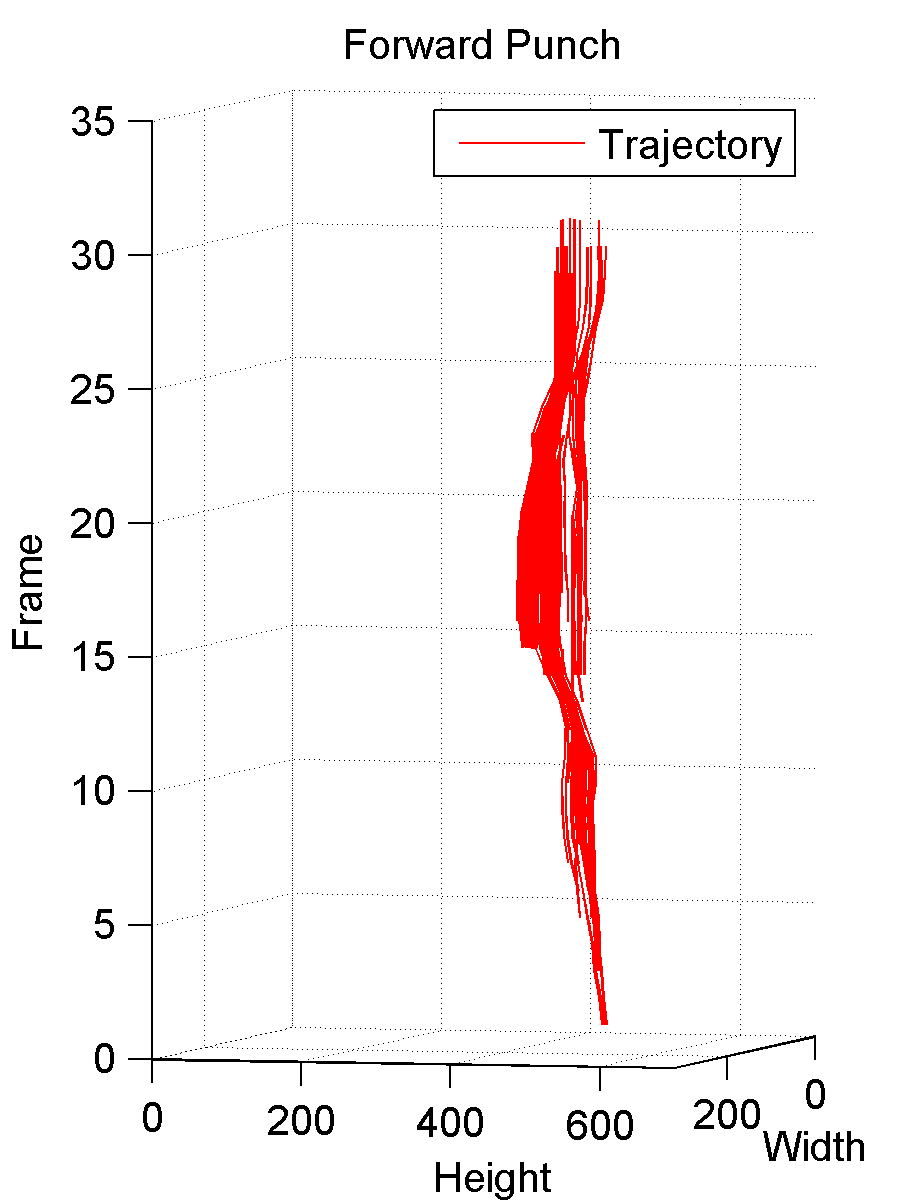
\includegraphics[scale=0.5]{ForwardPunch_TOP.png}
			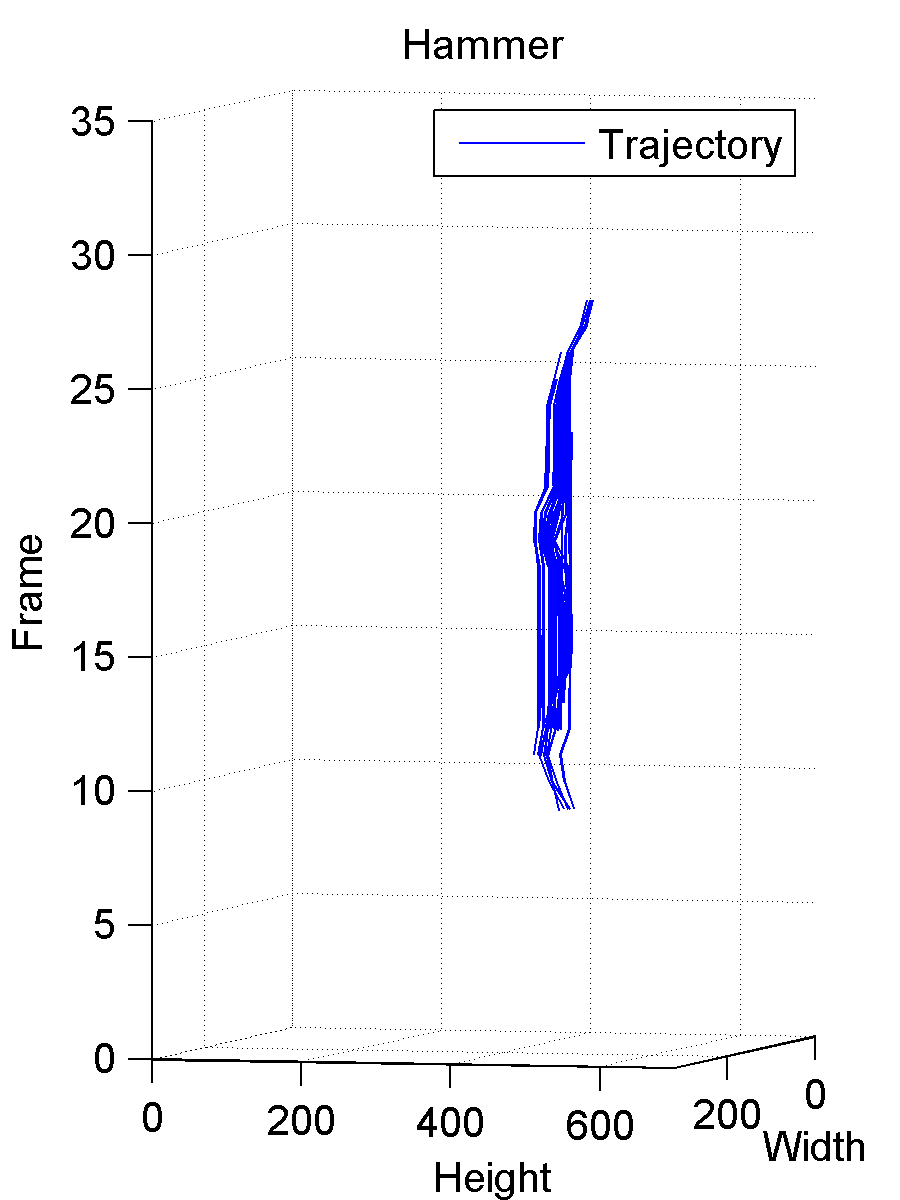
\includegraphics[scale=0.5]{Hammer_TOP.png}
		}
	\end{center}
	\caption{\label{fig:Illustration}Minh họa sự tương tự giữa phần lớn các Trajectories của 2 actions: Forward Punch \& Hammer.}
\end{figure}

\paragraph{Experiments and Results}Chúng tôi tiến hành các experiments trên challenging benchmark datasets, các kết quả thí nghiệm chỉ ra rằng phương pháp của chúng tôi đánh bại the SoA methods trên depth data. Các kết quả này đã cho thấy những contributions của our method: (1) We propose an adaptive method for 3D video representation by using 2D features. (2) We thực hiện comprehensive experiments on the state-of-the-art MSR Action 3D dataset and show that our method is the best when compared with the state-of-the-art 3D methods.

\paragraph{Paper structure}After a brief review of the related work in Section 2, the proposed method is described in Section 3. Section 4 presents the experimental results and their concerned discussions. The summaries of our work are given in Section 5.

\section{Related Works}

\subsection{Trajectories Extraction}
Trajectories provide a compact representation of motion information in video. Trajectories from intensity videos can be used for multimedia event detection (MED), video mining, action classification and so on. Trajectory extraction much depends on both processes: sampling and tracking. Some concerned methods, such as \cite{matikainen2009trajectons, messing2009activity} used KLT tracker \cite{lucas1981iterative}, or \cite{sun2009hierarchical} matched  SIFT descriptors between consecutive frames to obtain feature trajectories. Recently, the dense trajectories feature proposed by \cite{wang2011densetraj} has achieved state-of-the-art performances on MED systems, such as, segment-based system \cite{phan2014multimedia} on TRECVID MED 2010, 2011, or AXES \cite{oneata2012axes}, and BBNVISER \cite{natarajan2012bbn} on TRECVID MED 2012.

Although, depth data has been studied ago several decades, the trajectory extraction in depth videos is not still paid attention to. This is obviously a significant deficiency for motion feature-based systems using depth data.

\subsection{Feature Representation from Depth Videos}
In terms of human action recognition in depth video, most recent methods exploit depth information into two major directions. The first one is adapting intensity techniques-based methods for depth data. The second one is proposing approaches to use depth value as its mean.

For the first direction, Yang.X et al. \cite{yang2012recognizing} propose the Depth Motion Maps (DMM) to accumulate global activities in depth video sequences. And the Histogram of Oriented Gradients (HOG) are computed from the DMM to represent an action video. Another approach bases on spatio-temporal interest points proposed by Xia.L and Aggarwal.J.K \cite{xia2013spatio}. In this approach, they extend a work of Dollar et al. \cite{dollar2005behavior} to adapt for depth data.

For the second direction, \cite{li2010action} uses a bag of 3D points to characterize a set of salient postures. The 3D points are extracted on the contours of the planar projections of the 3D depth map. And then, about 1\% 3D points are sampled to calculate feature. \cite{vieira2012stop, wang2012robust, wang2012mining} use occupancy patterns to represent feature in action video. Another approach proposed by Oeifej et al. \cite{oreifej2013hon4d} leverages the distribution of surface normal orientation in the 4D space of time, depth and spatial coordinates to build a feature histogram. Inspired by results of Shotton et al. \cite{shotton2013real} and Xia.L et al. \cite{xia2011human}, works \cite{yang2012eigenjoints, wang2012mining} propose new types of features based on skeleton information.

Different from other approaches, we use a trajectory-based approach for action recognition. We do not care to segment human body like in \cite{li2010action,yang2012recognizing}. We only investigate the benefit of generating intensity representations from depth data, as mentioned in \cite{li2010action,yang2012recognizing}. Moreover, we leverage the effectiveness of trajectory feature to represent an action video. In our best knowledge, no methods has previously proposed for human action recognition using depth data. We conduct evaluations on recognition accuracy using dense trajectories motion feature proposed by Wang et al. \cite{wang2011densetraj}.

\section{Proposed Method}
This paper presents a effective depth video representation by adapting intensity trajectories-based motion features. First, chúng tôi sẽ cung cấp một brief review of the dense trajectories-based feature proposed by Heng Wang et al. \cite{wang2011densetraj}. Những phần liên quan như: dense sampling, tracking and feature descriptors is referred to. Our trajectories-based approach for depth data is mentioned at the end of this section.

\subsection{Dense trajectories}
% - Giới thiệu khái quát về dense trajectories
In order to obtain trajectories, there are two important steps: sampling and tracking. \cite{wang2011densetraj} propose sampling on a dense grid with a step size of 5 pixels. The sampling is performed at multiple scales with a factor of $1/\sqrt{2}$. Then, tracking is the next step to form trajectories. At each scale, in frame \textit{t}, each point \textit{$P_t = (x_t, y_t)$} is tracked to point \textit{$P_{t+1} = (x_{t+1}, y_{t+1})$} in next frame \textit{t+1} by:
\begin{equation}
	\textit{$P_{t+1} = (x_{t+1}, y_{t+1}) = (x_t, y_t) + (M*\omega)|_{(\bar{x}_t,\bar{y}_t)} $},
\end{equation}
where \textit{$\omega = (u_t, v_t)$} denotes the dense optical flow field, \textit{M} is the kernel of median filtering, and \textit{$(\bar{x}_t,\bar{y}_t)$} is the rounded position of \textit{$P_t$}. The algorithm of \cite{farneback2003two} is adopted to compute the dense optical flow. And to avoid a drifting problem, a suitable value of trajectory length is set to 15 frames. Beside, trajectories with sudden changes are removed.

After extracting trajectories, two kinds of descriptors: a trajectory shape descriptor and a trajectory-aligned descriptor can be adopted.

\paragraph{Trajectory Shape Descriptor}This descriptor describes the shape of a trajectory in the simplest way. Given a trajectory of length L, its shape is concatenated by a sequence of displacement vectors \textit{$S = (\Delta P_t, ..., \Delta P_{t+L-1})$}, where \textit{$\Delta P_t = P_{t+1} - P_t = (x_{t+1} - x_t, y_{t+1} - y_t)$}. In order to make the descriptor invariant to scale changes, the final result is then achieved by normalizing the shape vector by the overall magnitude of the displacement vectors:

\begin{equation}
	\textit{$\bar{S} = \frac{(\Delta P_t, ..., \Delta P_{t+L-1})}{\sum_{k=t}^{t+L-1}\|\Delta P_k\|}$},
\end{equation}

\paragraph{Trajectory-aligned Descriptor}The descriptors are much more complex than the trajectory shape descriptor. They are computed within a space-time volume ($N \times N$ spatial pixels and $L$ temporal frames) around the trajectory. This volume is divided into a 3D grid (spatially $n_\sigma \times n_\sigma$ grid and temporally $n_\tau$ segments). The default settings of these parameters are $N$ = 32 pixels, $L$ = 15 frames, $n_\sigma$ = 2, and $n_\tau$ = 3.

In order to capture the local motion and appearance around a trajectory, three kinds of descriptors have been employed: the Histogram of Oriented Gradient (HOG) \cite{dalal2005histograms}, the Histogram of Optical Flow (HOF) \cite{laptev2008learning}, and the Motion Boundary Histogram (MBH) \cite{dalal2006human}. For HOG, orientation information is quantized into 8-bin histogram. HOF is 9-bin histogram. Since the feature of a trajectory is calculated and concatenated from sub-volumes of a 3D volume, the final representation has 96 dimensions for HOG and 108 dimensions for HOF. MBH descriptor computes derivatives on both horizontal and vertical components of optical flow $I_\omega = (I_x. I_y)$. Similar to HOG descriptor, the orientation information is quantized into 8-bin histogram. Since the motion information is combined along two directions, the final representation is $96 \times 2 = 192$-bin histogram. By presenting gradient of optical flow, MBH descriptor is able to suppress global motion information and only keep local relative changes in pixels.

According to the authors \cite{laptev2008learning, wang2011densetraj, wang2009evaluation, liu2009recognizing}, all the three descriptors have shown the effectiveness for action recognition. The experimental settings for these descriptors are based on an empirical study showed in \cite{wang2011densetraj}. We also conduct our experiment on all the three descriptors when compared to the depth-based state-of-the-art methods.

\subsection{Pseudo-3D trajectory-based Approach for Motion Feature in Depth Data}

Our proposed trajectory-based approach for human action recognition in depth data is as follow. At first, intensity representations are formed from the sequence of depth maps, as illustrated in Figure 2. In particular, we choose number of the representations of 3. Number 3 represents 3 view directions: front, side, and top in 3D space. Forming the representations is necessary due to dimensional gap when we adapt 2D techniques for 3D data. After that, the dense trajectories are extracted from the intensity representations. And the feature descriptors are also computed in this step. At the next step, with each intensity representation, corresponding feature representation is quantized from raw trajectory features by apply a "bag-of-words" model. A "late fusion" scheme is used to generate the final feature representation for action in the sequence of depth maps (Fig. 3).

- Hình 2 - Illustration of proposed method - Depth maps -> 3 projections -> dense trajectories

- Hình 3 - Framework overview for our system - Depth data -> 3 feature extraction -> 3 BoW model -> 3 histogramintersection-SVM -> concatenated-score features -> cai-kernel SVM classifier

In order to generate intensity representations from the sequence of depth maps, we use the approach proposed in \cite{li2010action}. This technique is also used in \cite{yang2012recognizing}. Basically, this method projects depth maps onto three orthogonal planes in Casterian space to obtain corresponding intensity representations. However, motion representation for human action in the previous approaches is accumulated from global motion information. Therefore, these approaches must deal with the challenges from human segmentation problem in more complicated datasets. In contrast to the previous ones, we pay attention to capture local motion information for representing human actions. With the approach, we do not care the challenges for segmenting human body. To effectively use local motion information, we leverage the effectiveness of trajectory-based representation. In practice, we adopt the dense trajectory-based approach proposed in \cite{wang2011densetraj}. Thus, motion information in depth data can be reproduced by complementary motion information in different intensity representations.

Our proposed trajectory-based approach is compared with the state-of-the-art methods in human action recognition using depth data. Actually, our approach does not care skeleton extraction, which is used as an important factor in some works, such as \cite{wang2012mining, yang2012eigenjoints}. In fact, extracting skeleton exactly is still an unsolved problem, due to the challenges, such as: cluttered background, hardware quality, camera motion, ... Figure 4 illustrates an example case when extract skeleton information.

- Hình 4 - An example for skeleton extraction error.

\section{Experimental Settings}

\subsection{Dataset}
We test our method on MSR Action 3D dataset. This dataset contains 20 actions, as showed in Table \ref{lbl:20actions}. Actions are performed by ten subjects for two or three times in the context of game console interaction. In total, there are 567 sequences of depth maps. The depth maps are shot at frame rate of 15 fps. The size of the depth map is $640 \times 480$, we resize into $320 \times 240$ to ensure processing efficiency.

\begin{table}[H]
	\begin{center}
		% Table generated by Excel2LaTeX from sheet 'MSRAction3D names'
		\begin{tabular}{c|c|c|c}
		
		  {\bf   ID  } & {\bf Action Name} &   {\bf   ID  } & {\bf Action Name} \\
		\hline
		             1 &  high arm wave &             11 &  two hand wave \\
		
		             2 & horizontal arm wave &             12 &    side-boxing \\
		
		             3 &         hammer &             13 &           bend \\
		
		             4 &     hand catch &             14 &   forward kick \\
		
		             5 &  forward punch &             15 &      side kick \\
		
		             6 &     high throw &             16 &        jogging \\
		
		             7 &         draw x &             17 &   tennis swing \\
		
		             8 &      draw tick &             18 &   tennis serve \\
		
		             9 &    draw circle &             19 &     golf swing \\
		
		            10 &      hand clap &             20 & pick up \& throw \\
		
		\end{tabular}
	\end{center}
	\caption{\label{lbl:20actions}20 actions in MSR Action 3D dataset}
\end{table}

In order to conduct a fair comparison, we use the same experimental settings as \cite{li2010action, yang2012eigenjoints, yang2012recognizing, wang2012mining, xia2013spatio, oreifej2013hon4d}. In the settings, the dataset is divided into three action subsets. Each subset has 8 actions (Table \ref{lbl:3ActionSubsets}). The two subsets AS1 and AS2 present that grouped actions have similar movements. The subset AS3 groups complex actions together. For instance, action $hammer$ seems to be confused with action $forward punch$ in AS1 or similar movements between action $hand catch$ and action $side\ boxing$ in AS2. As for each subset, we select half of the subjects as training and the rest as testing (i.e. cross subject test).

\begin{table}[H]
	\begin{center}
		% Table generated by Excel2LaTeX from sheet 'Sheet3'
		\begin{tabular}{c|c|c}
		
		{\bf Action Subset 1} & {\bf Action Subset 2} & {\bf Action Subset 3} \\
		{\bf(AS1)} & {\bf(AS2)} & {\bf(AS3)} \\
		\hline
		horizontal arm wave &  high arm wave &     high throw \\
		
		        hammer &     hand catch &   forward kick \\
		
		 forward punch &         draw x &      side kick \\
		
		    high throw &      draw tick &        jogging \\
		
		     hand clap &    draw circle &   tennis swing \\
		
		          bend &  two hand wave &   tennis serve \\
		
		  tennis serve &    side-boxing &     golf swing \\
		
		pick up \& throw &   forward kick & pick up \& throw \\
		
		\end{tabular}
	\end{center}
	\caption{\label{lbl:3ActionSubsets}The three action subsets used in the experiments}
\end{table}

\subsection{Evaluation Method}

Figure 3 shows our evaluation framework for the trajectory-based features. We perform experiments using the proposed approach and compare with the state-of-the-art methods on depth data. We use the application available online\footnote{http://lear.inrialpes.fr/$\sim$wang/dense\_trajectories} to extract dense trajectories and aligned-features. To quantize a large number of features obtained by densely sampling, the "bag-of-words" (BoW) model is applied. At first, in each intensity representation, we randomly get about 80,000 extracted trajectories for clustering with K-mean algorithm. Then, a codebook of 2000 visual codewords is formed for each. After that, the hard-assignment technique is used to compute histograms of the visual words on the corresponding intensity representations.

Once all the BoW histograms are generated, we adopt the late-fusion scheme with the popular Support Vector Machine (SVM) for classification. In practice, we use the precomputed-kernel technique with the histogram intersection measurement for the first classification step and apply $\chi^2$ kernel for the next step. In our implementation, we use the libSVM library published online by author\footnote{http://www.csie.ntu.edu.tw/$\sim$cjlin/libsvm/} and perform the one-vs-all strategy for multi-class classification. We adopt the format requirements of the library to synchronize the annotation and the data. For testing, the scores of each intensity representation at the first classification step are concatenated to generate the final feature representation as the input of the final prediction. The predicted value is defined as the maximum score obtained from all the classifiers. This score shows that a human action is confused with another or not.

\section{Experimental Results}

This section presents the experimental results from applying our proposed approach on MSR Action 3D dataset. We also report the results on the main intensity representation (i.e. front projection). Beside, an evaluation related to selecting compensation information from other representations will be also mentioned. All the results are compared in terms of the accuracy. The best performance is highlighted in bold.

\subsection{Recognize Actions from An Intensity Representation}

Table \ref{lbl:MBHvsSoAonFront} - lists the results from our trajectory-based approach on front representation. Interestingly, the result table indicates that this approach beats all the state-of-the-art methods based on silhouette features \cite{li2010action, yang2012recognizing}, skeletal joint features \cite{yang2012eigenjoints, wang2012mining}, local occupancy patterns \cite{wang2012robust, vieira2012stop}, normal orientation features \cite{oreifej2013hon4d} and cuboid similarity features \cite{xia2013spatio}. However, the results also show that there is significant difference of the performance among the used feature descriptors.

\begin{table}[H]
	\begin{center}
		% Table generated by Excel2LaTeX from sheet 'Methods'
		\begin{tabular}{c|c}
		
		  {\bf Method} & {\bf Accuracy (\%)} \\
		\hline
		Bag of 3D Points [?] &         74.70  \\
		
		      STOP [?] &         84.80  \\
		
		EigenJoints [?] &         82.33  \\
		
		Random Occupancy Patterns [?] &         86.50  \\
		
		Local Occupancy Patterns [?] &         88.20  \\
		
		Depth Motion Maps-based HOG [?] &         91.63  \\
		
		Histogram of Oriented 4D Normals [?] &         88.89  \\
		
		Depth Cuboid Similarity Feature [?] &         89.30  \\
		\hline
		    {\bf Ours} &   {\bf 94.53 } \\
		
		\end{tabular}  
	\end{center}
	\caption{\label{lbl:MBHvsSoAonFront}Results on front representation using MBH descriptor.}
\end{table}

\begin{table}[H]
	\begin{center}
		% Table generated by Excel2LaTeX from sheet 'VIEWS_LateFusion'
		\begin{tabular}{ccc}
		
		       \multicolumn{ 3}{c}{{\bf Action Subsets}} \\
		\hline
		     {\bf AS1} &      {\bf AS2} &      {\bf AS3} \\
		\hline
		        92.45  &         92.04  &         99.11  \\
		
		\end{tabular}
	\end{center}
	\caption{\label{lbl:MBHandAS123}Results on three subsets.}
\end{table}

Consider the results on action subsets, we found that 2 subsets AS1, AS2 contain many confused actions (Table \ref{lbl:MBHandAS123}). For example, action-pair "hammer" and "forward punch" in AS1, or "side-boxing" and "hand catch" in AS2, as showed in Table \ref{lbl:AS123ConfusionMatrix}. When analyzing confused actions, we found that the main cause is due to similar movements. And, since depth data is textureless, it makes recognition more difficult. That is a reason why we need compensate information from other intensity representations.

\begin{table}[H]
	\begin{center}
		\subfloat[Action Subset 1 \label{lbl:ConfMatAS1}]{
			% Table generated by Excel2LaTeX from sheet 'Experiment-MSRDaily3D'
			\begin{tabular}{c|cccccccc}
			
			               &      {\bf a02} &      {\bf a03} &      {\bf a05} &      {\bf a06} &      {\bf a10} &      {\bf a13} &      {\bf a18} &      {\bf a20} \\
			\hline
			     {\bf a02} &   {\bf 0.833 } &              0 &   {\bf 0.167 } &              0 &              0 &              0 &              0 &              0 \\
			
			     {\bf a03} &              0 &   {\bf 0.917 } &   {\bf 0.083 } &              0 &              0 &              0 &              0 &              0 \\
			
			     {\bf a05} &              0 &   {\bf 0.364 } &   {\bf 0.636 } &              0 &              0 &              0 &              0 &              0 \\
			
			     {\bf a06} &              0 &              0 &              0 &     {\bf 1.0 } &              0 &              0 &              0 &              0 \\
			
			     {\bf a10} &              0 &              0 &              0 &              0 &     {\bf 1.0 } &              0 &              0 &              0 \\
			
			     {\bf a13} &              0 &              0 &              0 &              0 &              0 &     {\bf 1.0 } &              0 &              0 \\
			
			     {\bf a18} &              0 &              0 &              0 &              0 &              0 &              0 &     {\bf 1.0 } &              0 \\
			
			     {\bf a20} &              0 &              0 &              0 &              0 &              0 &   {\bf 0.067 } &              0 &   {\bf 0.933 } \\
			
			\end{tabular}
		}
		
		\subfloat[Action Subset 2 \label{lbl:ConfMatAS2}]{
			% Table generated by Excel2LaTeX from sheet 'Experiment-MSRDaily3D'
			\begin{tabular}{c|cccccccc}
			
			               &      {\bf a01} &      {\bf a04} &      {\bf a07} &      {\bf a08} &      {\bf a09} &      {\bf a11} &      {\bf a12} &      {\bf a14} \\
			\hline
			     {\bf a01} &     {\bf 1.0 } &              0 &              0 &              0 &              0 &              0 &              0 &              0 \\
			
			     {\bf a04} &   {\bf 0.083 } &   {\bf 0.833 } &   {\bf 0.083 } &              0 &              0 &              0 &              0 &              0 \\
			
			     {\bf a07} &              0 &              0 &   {\bf 0.786 } &   {\bf 0.071 } &   {\bf 0.071 } &              0 &   {\bf 0.071 } &              0 \\
			
			     {\bf a08} &              0 &              0 &              0 &     {\bf 1.0 } &                &              0 &              0 &              0 \\
			
			     {\bf a09} &              0 &              0 &              0 &   {\bf 0.133 } &   {\bf 0.867 } &              0 &              0 &              0 \\
			
			     {\bf a11} &              0 &              0 &              0 &              0 &              0 &     {\bf 1.0 } &              0 &              0 \\
			
			     {\bf a12} &              0 &   {\bf 0.133 } &              0 &              0 &              0 &              0 &   {\bf 0.867 } &              0 \\
			
			     {\bf a14} &              0 &              0 &              0 &              0 &              0 &              0 &              0 &     {\bf 1.0 } \\
			
			\end{tabular}
		}
		
		\subfloat[Action Subset 3 \label{lbl:ConfMatAS3}]{
			% Table generated by Excel2LaTeX from sheet 'Experiment-MSRDaily3D'
			\begin{tabular}{c|cccccccc}
			
			               &      {\bf a06} &      {\bf a14} &      {\bf a15} &      {\bf a16} &      {\bf a17} &      {\bf a18} &      {\bf a19} &      {\bf a20} \\
			\hline
			     {\bf a06} &     {\bf 1.0 } &              0 &              0 &              0 &              0 &              0 &              0 &              0 \\
			
			     {\bf a14} &              0 &     {\bf 1.0 } &              0 &              0 &              0 &              0 &              0 &              0 \\
			
			     {\bf a15} &              0 &              0 &     {\bf 1.0 } &              0 &              0 &              0 &              0 &              0 \\
			
			     {\bf a16} &              0 &              0 &              0 &     {\bf 1.0 } &              0 &              0 &              0 &              0 \\
			
			     {\bf a17} &              0 &              0 &              0 &              0 &     {\bf 1.0 } &              0 &              0 &              0 \\
			
			     {\bf a18} &              0 &              0 &              0 &              0 &              0 &   {\bf 0.933 } &   {\bf 0.067 } &              0 \\
			
			     {\bf a19} &              0 &              0 &              0 &              0 &              0 &              0 &     {\bf 1.0 } &              0 \\
			
			     {\bf a20} &              0 &              0 &              0 &              0 &              0 &              0 &              0 &     {\bf 1.0 } \\
			
			\end{tabular}
		}
		
	\end{center}
	\caption{\label{lbl:AS123ConfusionMatrix}Confusion matrices on three subsets.}
\end{table}

\subsection{Compensate Motion Information from Other Representations}
 
 Trong phần thí nghiệm này, chúng tôi bổ sung thông tin từ các representation còn lại cho representation ban đầu. Figure \ref{lbl:Figure_LateFusion_AS123_MBH} chỉ ra a better view khi so sánh hiệu quả của Fusion với các separate representations. Expectedly, the fusion performance, which is 0.9543 accuracy, is better than all the separate ones on each representation in terms of average. Obviously, our proposed approach outperforms the mentioned state-of-the-art methods.
 
 \begin{figure}[H]
 	\begin{center}
 		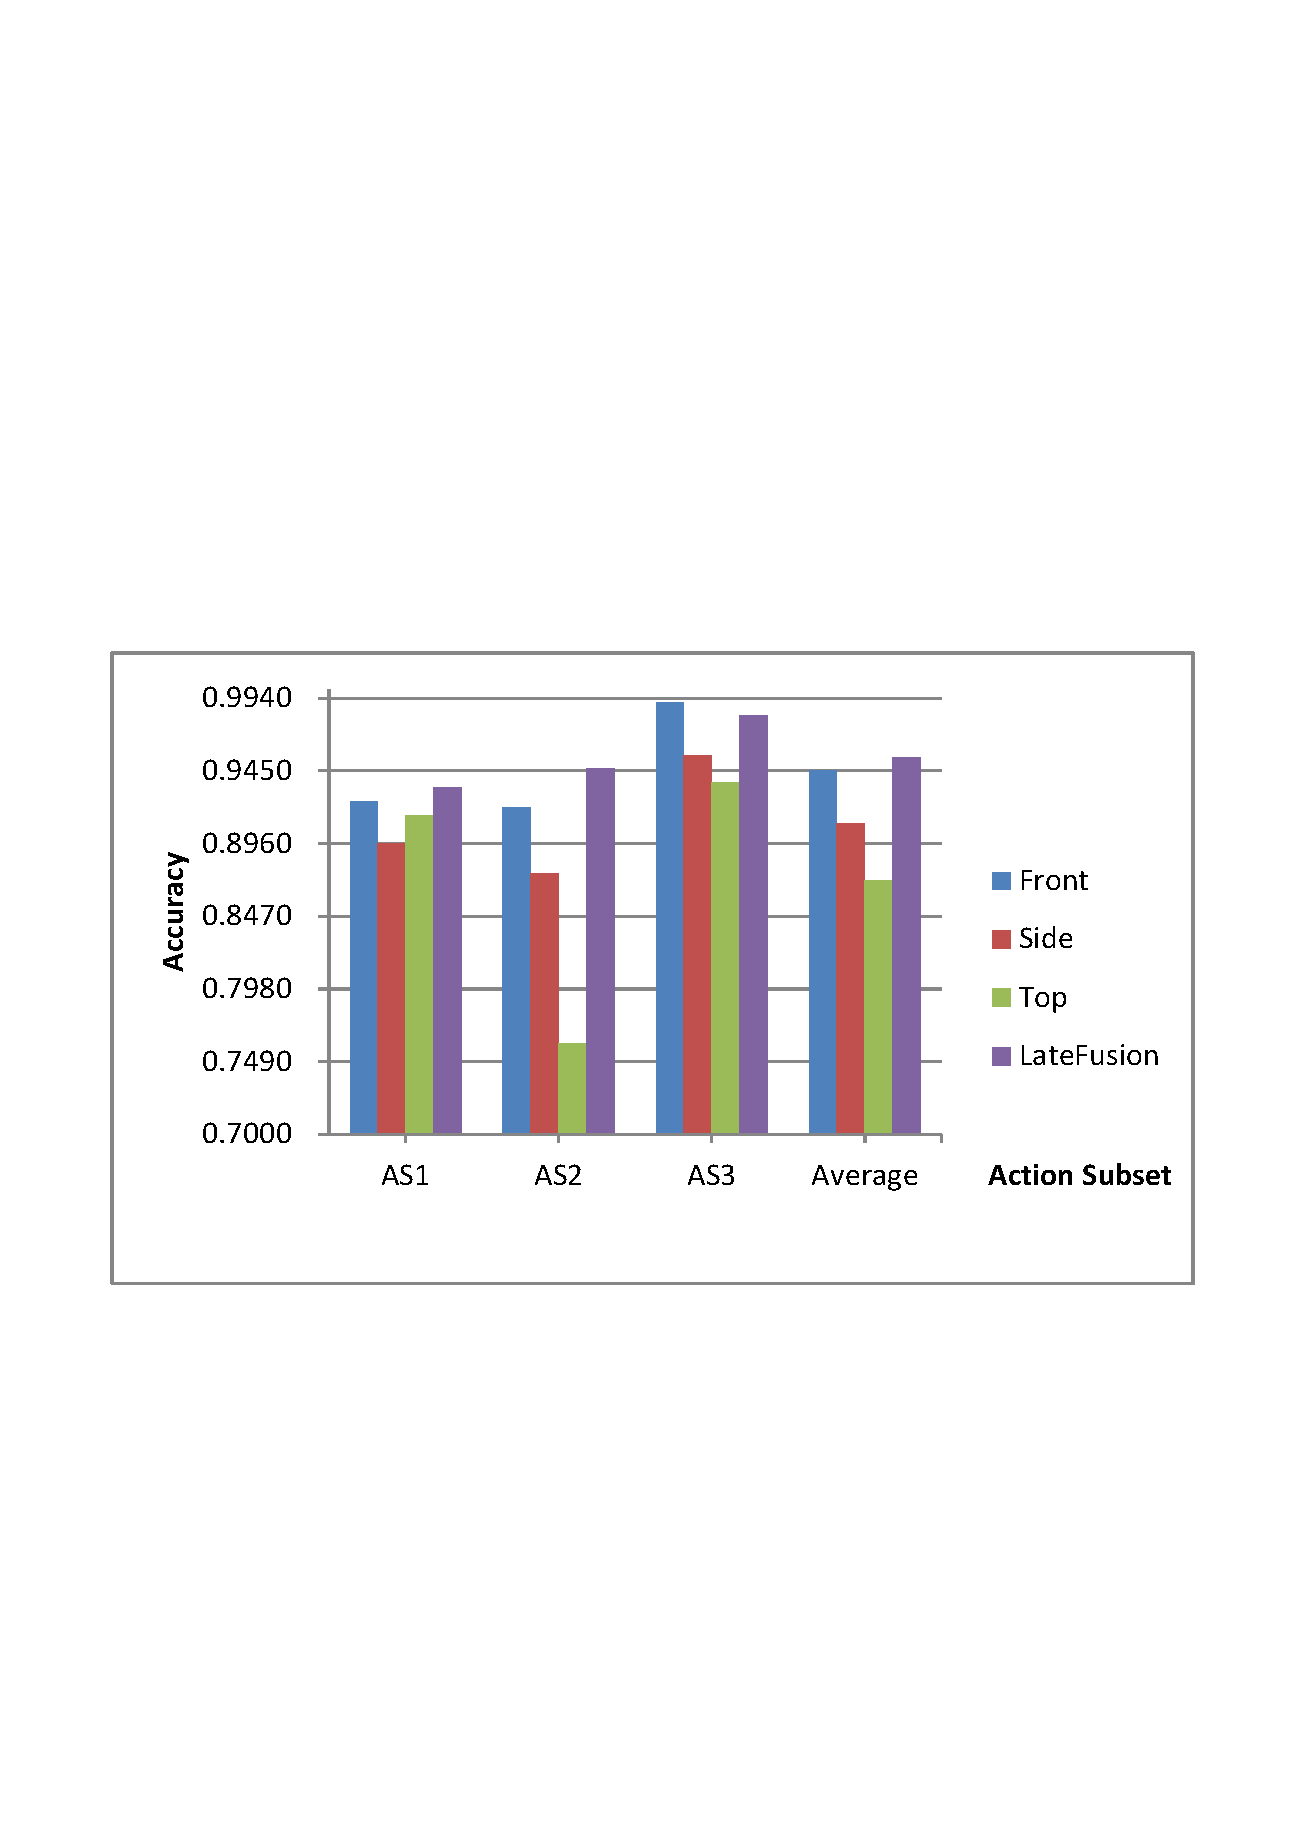
\includegraphics[scale=0.6]{Chart_LateFusion_AS123_MBH.eps}
 	\end{center}
 	\caption{\label{lbl:Figure_LateFusion_AS123_MBH}Results from using the late fusion scheme on representations}
 \end{figure}
 
Ngoài ra, dựa vào kết quả được chỉ ra ở Figure \ref{lbl:Figure_LateFusion_AS123_MBH}, việc bổ sung thông tin từ các representations khẳng định 2 điều. The first one bảo đảm rằng kết quả nhận biết từ front representation là đóng vai trò quan trọng nhất. The second one chỉ ra rằng thông tin bổ sung từ các represenations khác có thể hỗ trợ hiệu quả cho final predictions.

\section{Discussions}

\subsection{Evaluate the Role of Intensity Representations}

Trong phần này, chúng tôi muốn thảo luận về vai trò của các representations trong cách tiếp cận của chúng tôi. Figure \ref{lbl:Figure_LateFusion_AS123_MBH} khẳng định rằng front representation luôn cho kết quả nhận biết tốt nhất so với phần còn lại. Rõ ràng, nó là thành phần không thể thiếu trong việc tổng hợp thông tin. Đối với phần còn lại, chúng tôi thực hiện thử nghiệm trên các tổ hợp representations với front representation. Kết quả thử nghiệm được chỉ ra ở Figure \ref{lbl:Figure_CombinationsFRONTSIDETOP}.

\begin{figure}[H]
	\begin{center}
		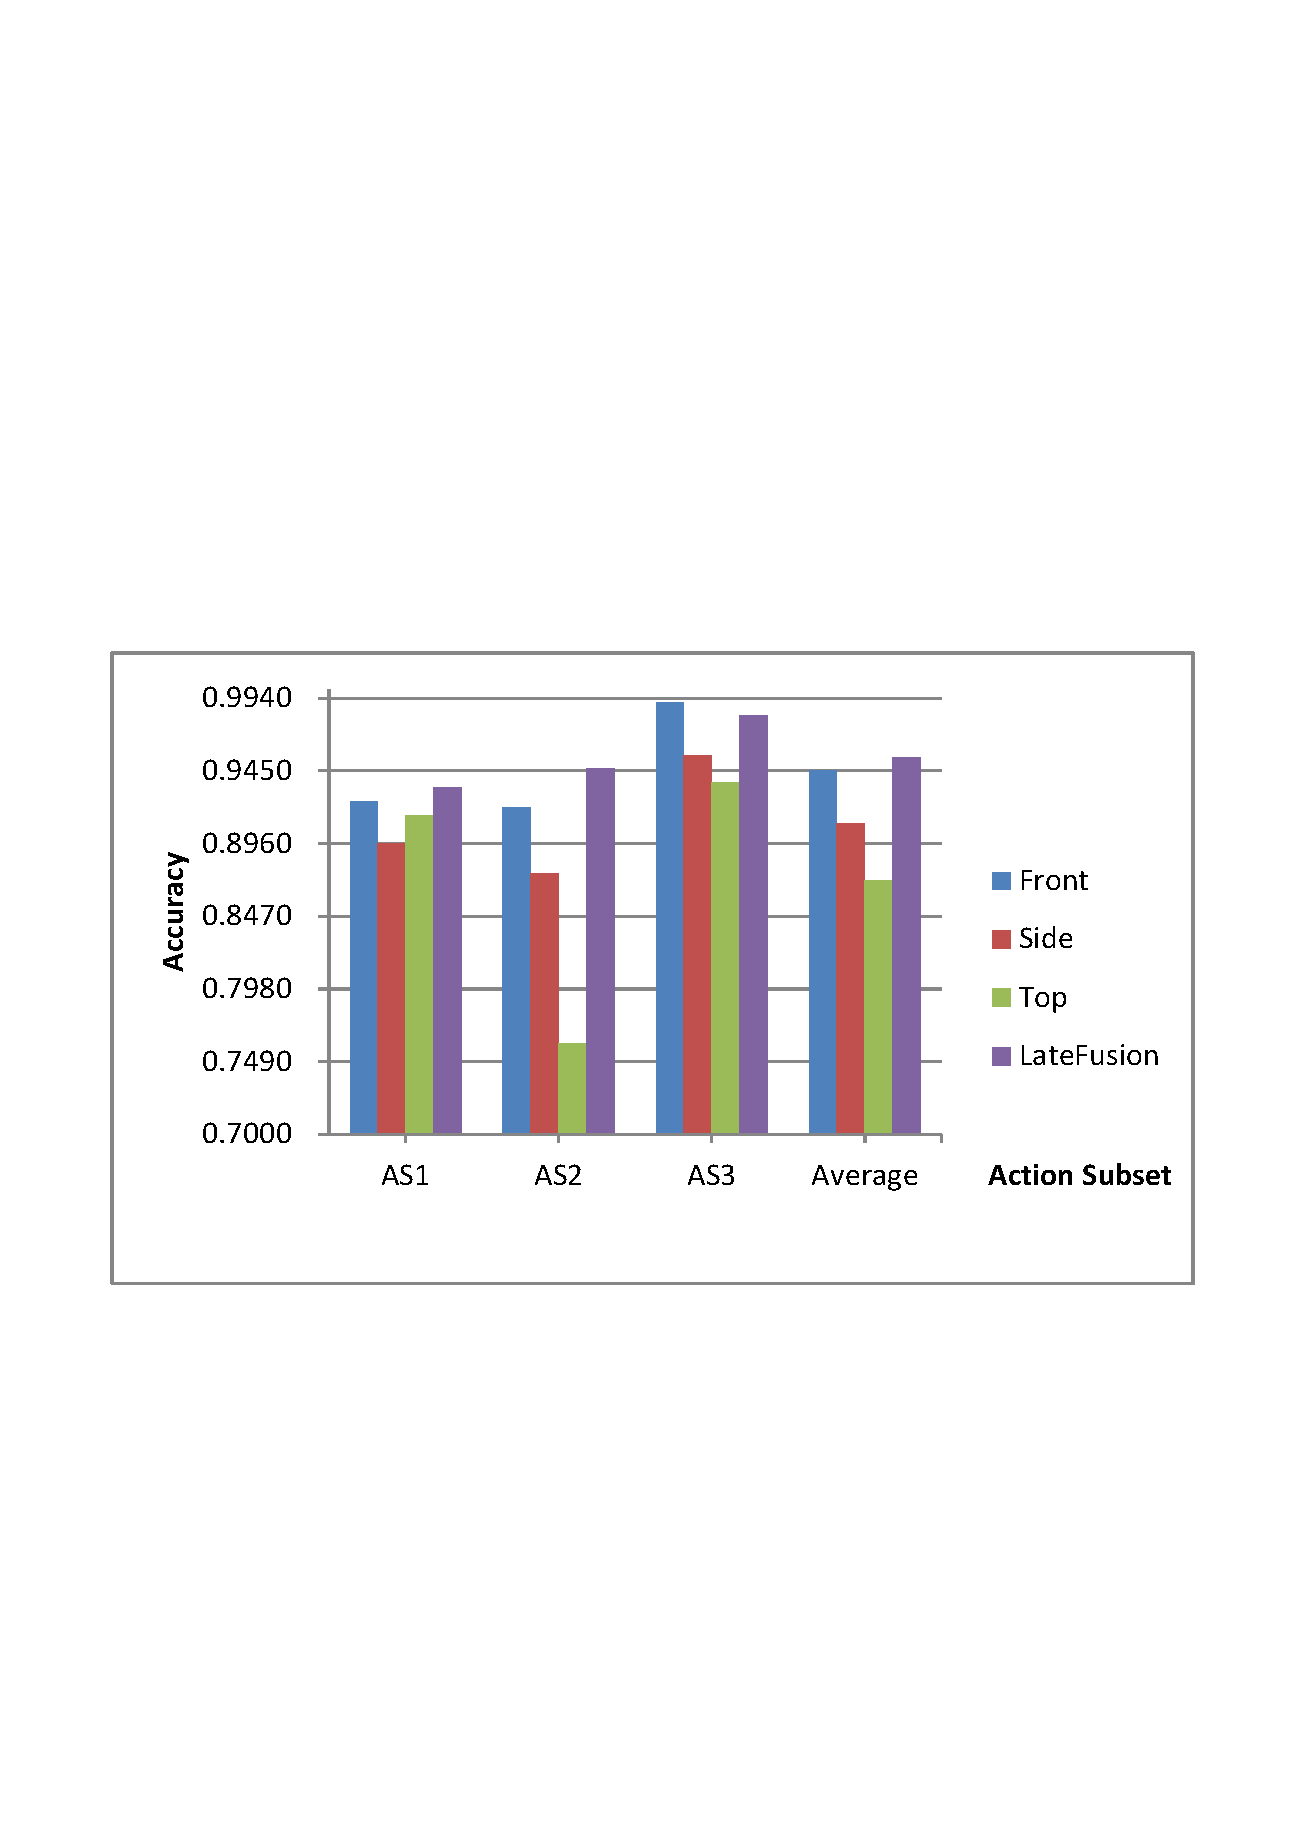
\includegraphics[scale=0.5]{Chart_LateFusion_AS123_MBH.eps}
	\end{center}
	\caption{\label{lbl:Figure_CombinationsFRONTSIDETOP}Results on combinations of representations}
\end{figure}

Trong phần thí nghiệm này, chúng tôi tạo ra các tổ hợp representations: front and Side, front and Top. Kết quả cho thấy khi tổ hợp front and top là tốt hơn hẳn so với tổ hợp front and side . Thậm chí, kết quả này là comparable with kết quả của việc tổ hợp all the representations. Rõ ràng, nếu chúng ta quan tâm đến chi phí tính toán thì việc chỉ dựa vào tổ hợp gồm ít representations hơn nhưng vẫn đảm bảo performance là lựa chọn hàng đầu. Đây là kết quả rất có ý nghĩa mà các ứng dụng xử lý thực tế luôn hướng đến.

\subsection{The Impact of Our Method on Descriptors}

Trong dữ liệu intensity, according to \cite{wang2011densetraj} MBH is the best feature descriptor for dense trajectories. Therefore, trong các thí nghiệm trước, chúng tôi chỉ sử dụng MBH descriptor cho việc biểu diễn motion information. Tuy nhiên, do bởi sự khác biệt của depth data với intensity data, thì cách tiếp cận của chúng tôi có ảnh hưởng như thế nào đối với các khác trajectory-aligned descriptors (i.e. HOG, HOF). Trong phần này, chúng tôi sẽ present lại các kết quả thí nghiệm nhưng trên các descriptors này.

\begin{figure}[H]
	\begin{center}
		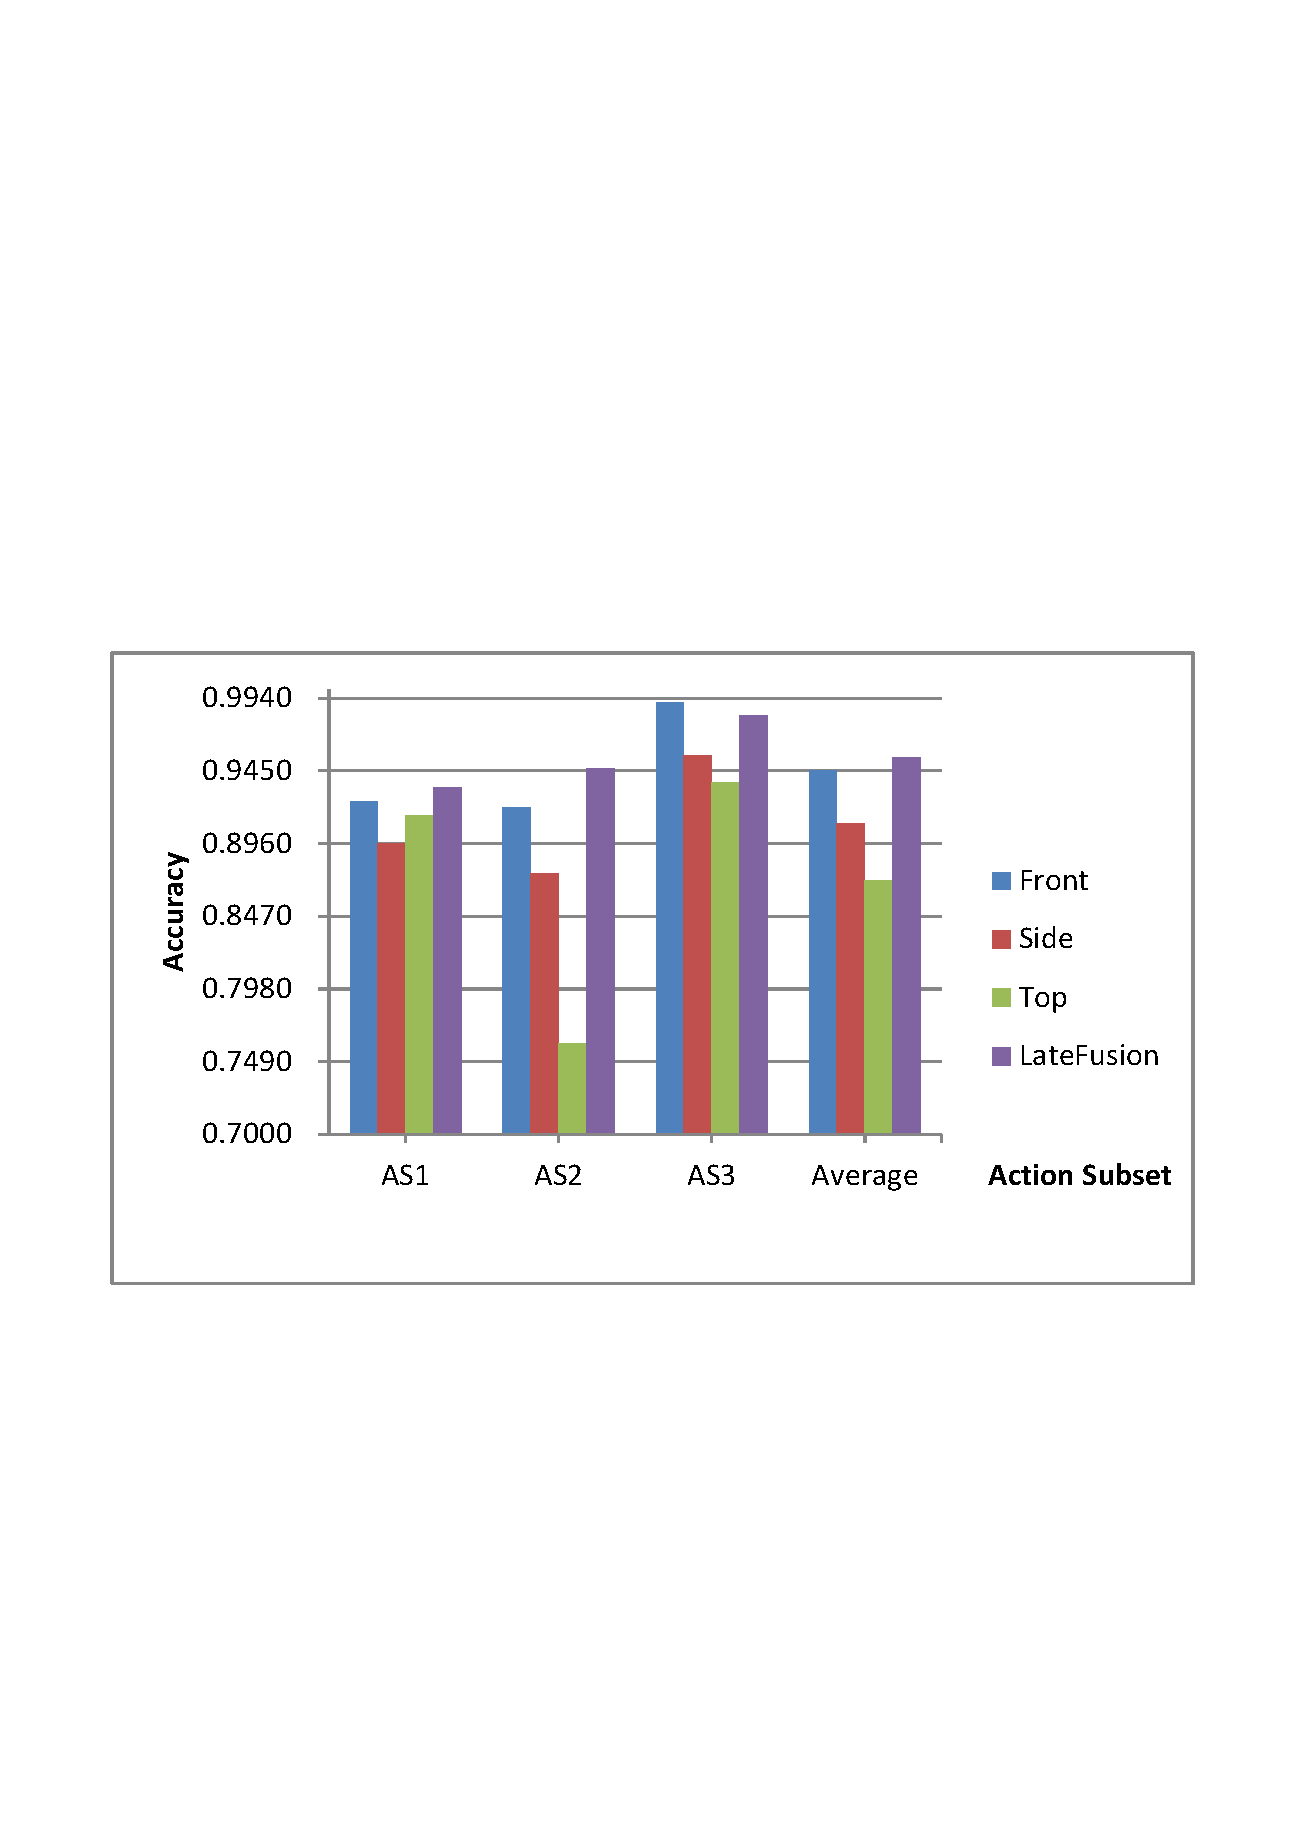
\includegraphics[scale=0.5]{Chart_LateFusion_AS123_MBH.eps}
	\end{center}
	\caption{\label{lbl:Figure_MBHHOGHOF}Results on trajectory-aligned descriptors}
\end{figure}

Figure \ref{lbl:Figure_MBHHOGHOF} shows ra một kết quả rất interesting. Mặc dù, kết quả nhận biết của các descriptors HOG, HOF là không tốt trên mỗi intensity representation, kết quả sau khi fusion đã được improve đáng kể. The fusion results cho thấy HOG, HOF cũng outperform the state-of-the-art methods like MBH. Beside, HOG, HOF lại rất có lợi trong việc giảm thiểu chi phí tính toán trong các bước như: feature extraction and representation (using the bag-of-words model). This issue means rằng với các descriptors đơn giản hơn chúng ta không những xây dựng được một hệ thống effective mà còn efficient. It is worth to apply for real processing systems.

\section{Conclusions}

We proposed using the trajectory-based approach for human action recognition using depth data in this work. We evaluated our approach by using the dense trajectories motion feature on MSR Action 3D datasets. More interestingly, our proposed trajectory-based approach only applied for one representation beats all the recent state-of-the-art approaches in terms of depth data. Beside, in order to deal with confused actions due to similar movements, compensating information from other representations is proposed. Therefore, the effectiveness of our approach on depth datasets like MSR is confirmed.

A trajectory-based approach with compensating information from separate representations shows promising results. This opens a general approach to leverage intensity-based techniques for depth data. This also suggests the importance of trajectory-based motion information on human action recognition using depth data. Therefore, exploiting depth-trajectory-based motion information for human action can be beneficial for an action recognition system. This is also an interesting idea for our future work.

\section*{References}

\bibliographystyle{splncs}
\bibliography{JournalPaper_Ref}

\end{document}